\utsection{OpenBTS Software-Architektur}{Stefan Giggenbach}\label{sec:swarch}

\subsection{Überblick}

OpenBTS ist vollständig in der objektorientierten Sprache C++ implementiert. Dabei wird ein modularer Aufbau verwendet, der die wichtigsten Bestandteile des Systems logisch zusammenfasst. Folgende Auflistung zeigt die einzelnen Module von OpenBTS, die der Ordnerstrutkur im Verzeichnis \lstinline{<openbts>/src/openbts/trunk} entspricht.

\begin{itemize}
 \item \textit{apps} - OpenBTS Applikation (main-File)
 \item \textit{CLI} - Command Line Interface
 \item \textit{CommonLibs} - Standardfunktionen wie BitVector, Sockets, Thread, etc.
 \item \textit{Control} - Funktionen für GSM Call Control, Mobility Management und SIP
 \item \textit{Globals} - Deklaration der globalen Variablen
 \item \textit{GSM} - GSM Stack
 \item \textit{SIP} - SIP State Machine die vom Control Modul verwendet wird
 \item \textit{SMS} - SMS Stack
 \item \textit{sqlite3} - SQLite3 Zugriffsfunktionen
 \item \textit{SR} - Subscriber Registry
 \item \textit{Transceiver} - Software Transceiver mit Ünterstützung des USRP1
 \item \textit{TRXManager} - Schnittstelle zwischen GSM Stack und Software Transceiver
\end{itemize}

Das \textit{apps}-Modul stellt die eigentliche OpenBTS Applikation dar. Neben dem ausführbaren Binary befindet sich in diesem Verzeichnis mit der Datei \lstinline{OpenBTS.cpp} das main-File des Projekts. In dieser Datei werden alle verwendeten globalen Objekte instanziiert, die Konfiguration der benötigten Ressourcen durchgeführt und die am Programmablauf beteiligten Threads gestartet. Neben dem \textit{apss}-Modul werden sowohl das \textit{CLI}- als auch das \textit{GSM}-Modul, für die Erweiterung der Software um die Handover-Funktionalität, modifiziert. Die restlichen Module und deren Funktion werden nur aus Gründen der Vollständigkeit aufgeführt.

In den beiden folgenden Abschnitten werden zwei Klassen des GSM-Moduls, die bei der Implementierung der Handover-Funktionalität eine wichtige Rolle spielen, genauer betrachtet.

\subsection{LogicalChannel-Klassen}

Bei einem Intra BSC Handover werden, wie bereits in Abschnitt \ref{sec:handover} beschrieben, mit dem SACCH, dem TCH und dem FACCH drei verschiedene GSM-Kanaltypen verwendet. Im Quellcode von OpenBTS werden diese Kanaltypen von der Superklasse \lstinline{LogicalChannel} abgeleitet. In Abbildung \ref{fig:logchan} sind neben dieser Superklasse die beiden abgeleiteten Klassen \lstinline{TCHFACCHLogicalChannel} und \lstinline{SACCHLogicalChannel} exemplarisch für alle anderen Kanaltypen dargestellt. Das Klassendiagramm zeigt nur die bei der Implementierung verwendeten Methoden und bildet daher nicht die vollständige Klassenstruktur ab. Die Definition und Implementierung der Klassen befinden sich in den Dateien \lstinline{GSMLogicalChannel.h} und \lstinline{GSMLogicalChannel.cpp} des GSM-Moduls.

\begin{figure}[h!]
  \centering
  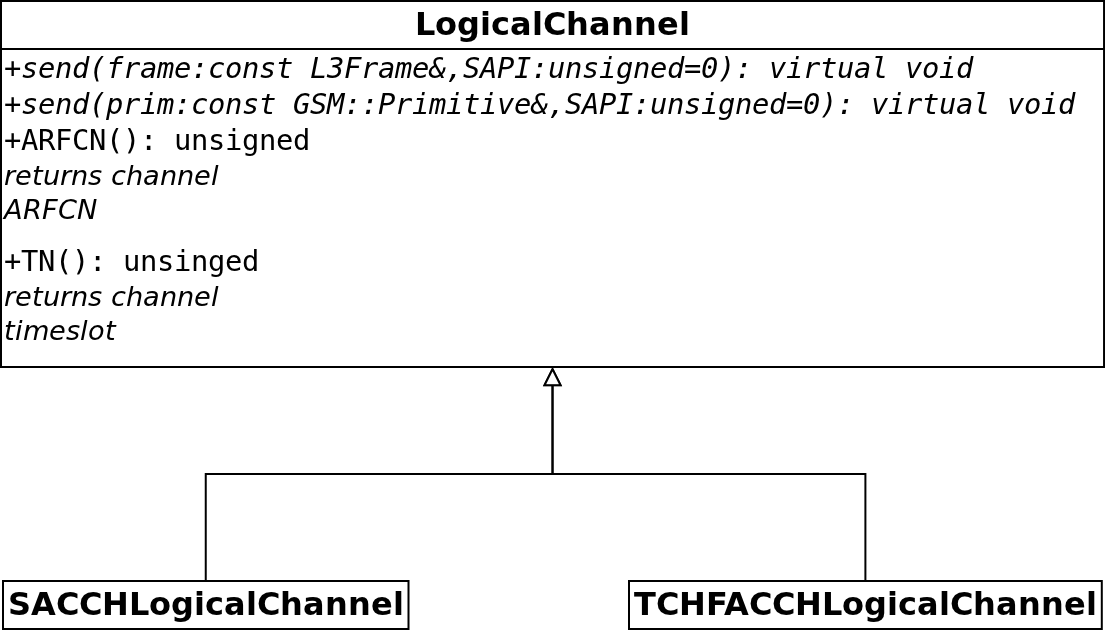
\includegraphics[width=0.7\textwidth]{img/lc}
  \caption{Klassendiagramm LogicalChannel}
  \label{fig:logchan}
\end{figure}

Alle im Handover-Modul verwendeten Methoden sind bereits in der Superklasse \lstinline{LogicalChannel} implementiert. Sie werden an der entsprechenden Stelle des Programmablaufs allerdings über Objekte des Typs \lstinline{SACCHLogicalChannel} bzw. \lstinline{TCHFACCHLogicalChannel} aufgerufen. Die Methoden \lstinline{TN()} und \lstinline{ARFCN()} geben die vom jeweiligen Kanal verwendete Frequenz (ARFCN) bzw. den verwendeten Timeslot (TN) zurück. Die beiden Methoden dienen damit primär zur Idenfikation und Zuordnung der Kanäle zu einem aktiven Gespräch (siehe Abschnitt \ref{sec:hom}).

Die beiden \lstinline{send()}-Methoden unterscheiden sich nur in ihrer Signatur und werden verwendet um Daten im jeweiligen Kanal zu transportieren. Einer Methode kann dabei ein selbst erzeugter Layer 3 Frame übergeben werden, der anschließend versendet wird (mehr dazu im folgenden Abschnitt). Die zweite Methode erlaubt das Senden von bereits im OpenBTS-Quellcode implementierten GSM-Primitven, wie der Freigabe eines Kanals mit der Primitive \lstinline{GSM::RELEASE}.

\subsection{L3Message-Klassen}

Ein wichtiger Vorgang während des Ablaufs eines Intra BSC Handover ist das senden des Handover-Command innerhalb des FACCH der bestehenden Verbindung. Das Kommando wird mit der bereits vorgestellten \lstinline{send()}-Methode des entsprechenden \lstinline{TCHFACCHLogicalChannel}-Objekts gesendet. Das eigentlich Kommando und dessen Inhalt muss allerdings erst erzeugt werden. Abbildung \ref{fig:l3mess} zeigt das Klassendiagramm der während der Projektarbeit implementierten Klasse \lstinline{L3HandoverCommand} und die entsprechenden Superklassen. Die Definition und Implementierung der Klasse erfolgt in den Dateien \lstinline{GSML3RRMessages.h} und \lstinline{GSML3RRMessages.cpp} des GSM-Moduls.

\begin{figure}[h!]
  \centering
  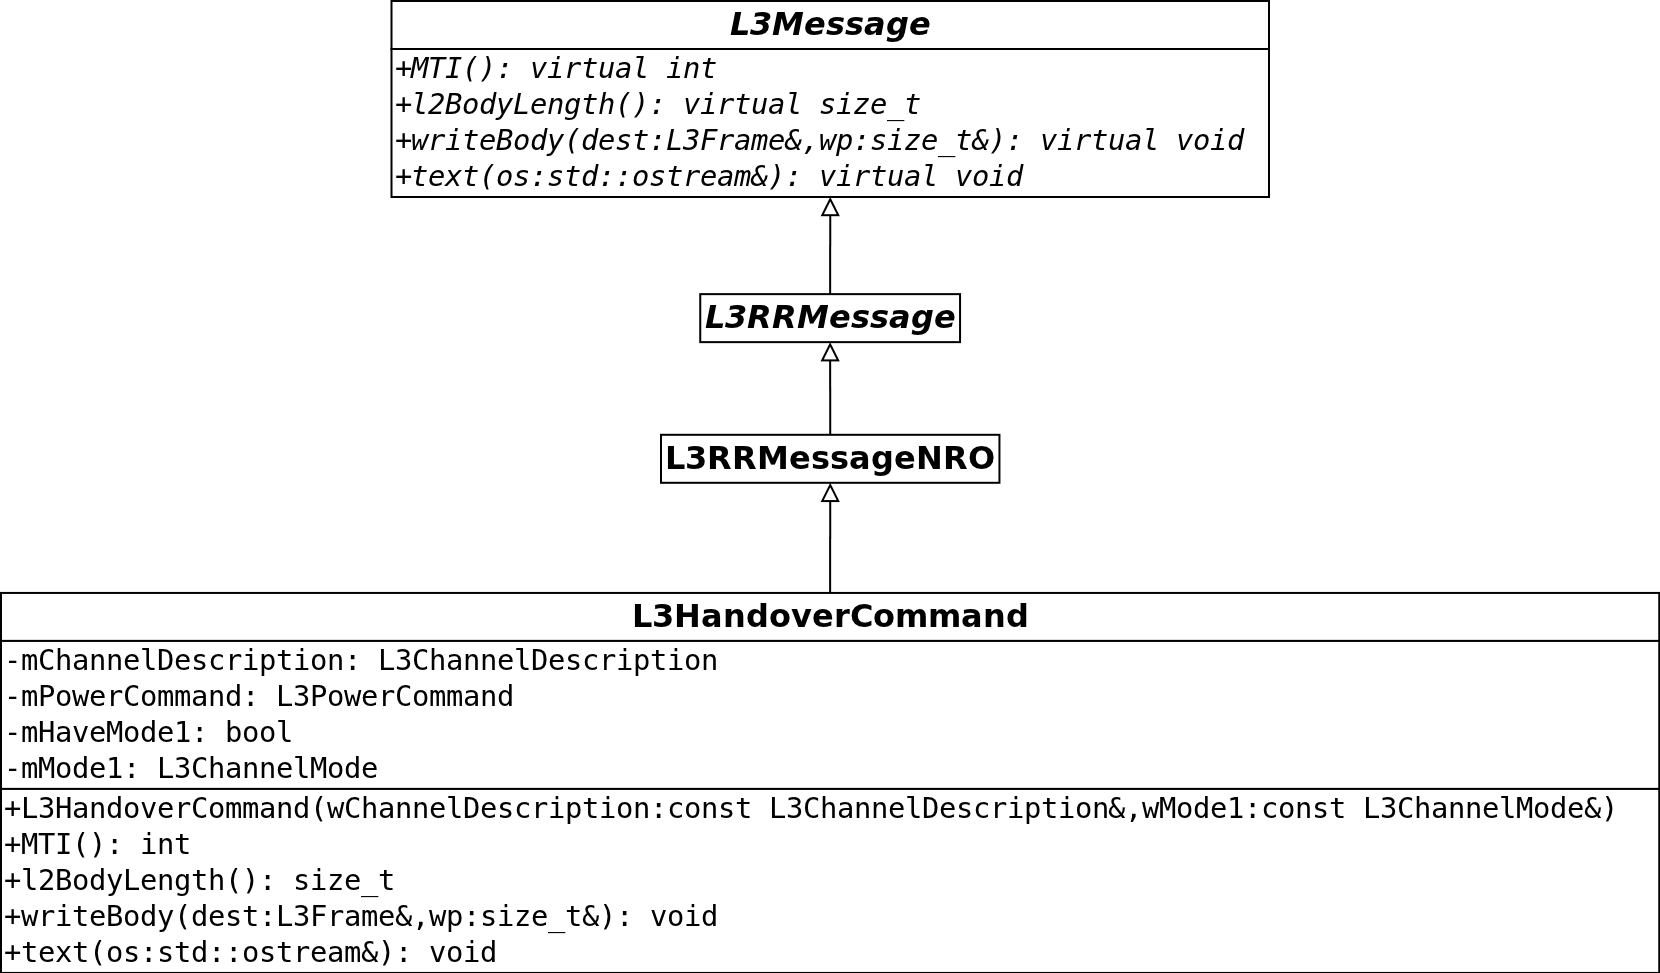
\includegraphics[width=\textwidth]{img/l3m}
  \caption{Klassendiagramm L3Message}
  \label{fig:l3mess}
\end{figure}

Dem Konstruktor der \lstinline{L3HandoverCommand}-Klasse wird als erster Parameter eine Referenz auf das \lstinline{TCHFACCHLogicalChannel}-Objekt des neuen TCH übergeben. Aus diesem Objekt werden, mit den bereits vorgestellten Methoden, sowhol die Frequenz als auch der Timeslot für das Handover-Command extrahiert. Der zweite Parameter ist der Channel-Mode, der bei den durchgeführten Tests immer dem Typ \lstinline{GSM::L3ChannelMode(GSM::L3ChannelMode::SpeechV1)} entspricht. Die drei restlichen Methoden werden automatisch beim Senden bzw. Erzeugen des Kommandos aufgerufen. Die Methode \lstinline{MTI()} gibt dabei den Message Type Indicator des Handover-Command zurück. Die Methode \lstinline{writeBody()} erzeugt den als Parameter übergebenen Layer 3 Frame der anschließend mit der \lstinline{send()}-Methode gesendet wird. Dabei ist darauf zu achten das bei der Implementierung der \lstinline{writeBody()}-Methode die Größe der einzelnen Blöcke in Bit angegeben werden muss. Im Gegensatz dazu gibt die Methode \lstinline{l2BodyLength()} die Länge des Frames in Byte zurück. Die \lstinline{text()}-Methode erzeugt lediglich eine lesbare Ausgabe des Kommandos und ist für die Funktion nicht entscheidend.
